Vamos a introducir una última mejora en la forma en la que generamos la imagen. Un defecto típico en computación gráfica es el conocido como \textbf{\textit{aliasing}}. Este se caracteriza por la presencia de dientes de sierra en lineas curvas o diagonales, y en nuestro caso se puede apreciar muy fácilmente en los bordes del cubo y en la cuadrícula del suelo en la distancia (\autoref{subfig:noAA}). En el mercado actual existen multitud de alternativas como solución a este problema. Algunos ejemplos son FXAA, basado en espacio de pantalla, o SSAA y MSAA, que usan la técnica del \textbf{supermuestreo} o \textbf{\textit{supersampling}} junto con filtros de suavizado. Nosotros implementaremos una versión de SSAA (\textit{Supersampling Anti-Aliasing}), pero antes debemos entender por qué aparece el problema del \textit{aliasing} en primer lugar. \newline

Toda pantalla tiene resolución finita, y por tanto la definición con la que puede mostrar la información es limitada. Al realizar la proyección sobre la pantalla puede ocurrir que una primitiva no ocupe un píxel completo, y como cada píxel solo puede mostrar un único color hay que elegir algún criterio para determinar qué hacer en esos casos. El más común es considerar que el píxel pertenece a la primitiva si su proyección cubre el centro del píxel. En nuestro caso esto se traducía en trazar el rayo a través del centro del píxel en el algoritmo de \textit{spheretracing}. Al hacer esta aproximación es cuando aparecen los dientes de sierra, pues a no ser que se trate de una línea totalmente vertical u horizontal, es como si intentásemos construir una rampa con escalones.\newline

Lo cierto es que no podemos hacer desaparecer este problema, pues es algo intrínseco de la naturaleza discreta de las pantallas y los sistemas de muestreo. En nuestro caso esto último se traduce en que no podemos trazar infinitos rayos. No obstante, lo que sí podemos hacer es tratar de disimularlo. En lugar de tomar una decisión binaria de si un píxel debe ser de un color u otro podemos intentar tener en cuenta la aportación de otras primitivas que estén cercanas dentro del píxel aunque no ocupen su centro. Una primera idea podría ser que una vez asignado un color a un píxel se hiciera la media con sus píxeles vecinos para así generar una transición suave entre ellos. Sin embargo este acercamiento presenta dos grandes inconvenientes:
\begin{itemize}
    \item Estaríamos perdiendo parte de la información original, y por ende, haciendo la imagen más borrosa.
    \item El responsable de asignar el color de cada píxel es una instancia del \textit{fragment shader}, y como ya comentamos, los \textit{shaders} son programas independientes y no tienen información sobre el resto de instancias. Por tanto este método sería de postprocesado, es decir, sería ejecutado una vez hubiera sido generada la imagen.
    
\end{itemize}

De esto podemos sacar la conclusión de que la solución debe ser local a cada píxel, y de ser posible que no conlleve la pérdida de información. La opción de hacer una media entre varias muestras de píxeles sigue pareciendo razonable, lo que nos lleva a la idea detrás de SSAA: tomar más muestras dentro de cada píxel. Para ello, tendremos que trazar rayos por más puntos dentro del píxel, esto es, dibujar la imagen con mayor resolución, de donde viene el nombre de supermuestreo. El patrón en el que tomamos las nuevas muestras es de nuestra elección. En la \autoref{fig:patrones} se muestran algunos patrones comunes, de los cuales optaremos por el uniforme por su sencillez y porque proporciona resultados bastante buenos en general. El número de evaluaciones también está a nuestra elección, pero no hay que olvidar el factor del rendimiento, ya que usando este patrón el número de rayos crece exponencialmente por cada nuevo nivel adicional de precisión.
\newline

\begin{figure}[htbp]
    \centering
    \begin{subfigure}[b]{0.25\textwidth}
        \centering
        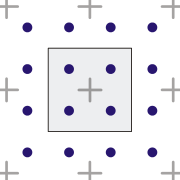
\includegraphics[width=\textwidth]{Plantilla-TFG-master/img/aa1.png}
        \caption{Uniforme}
    \end{subfigure}
    \hfill
    \begin{subfigure}[b]{0.25\textwidth}
        \centering
        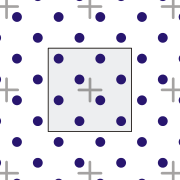
\includegraphics[width=\textwidth]{Plantilla-TFG-master/img/aa2.png}
        \caption{Rejilla girada}
    \end{subfigure}
    \hfill
    \begin{subfigure}[b]{0.25\textwidth}
        \centering
        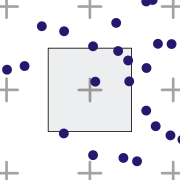
\includegraphics[width=\textwidth]{Plantilla-TFG-master/img/aa3.png}
        \caption{Aleatorio}
    \end{subfigure}
    
    \medskip
    
    \begin{subfigure}[b]{0.25\textwidth}
        \centering
        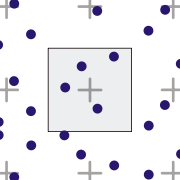
\includegraphics[width=\textwidth]{Plantilla-TFG-master/img/aa4.png}
        \caption{\textit{Quasi-Monte Carlo}}
    \end{subfigure}
    \hfill
    \begin{subfigure}[b]{0.25\textwidth}
        \centering
        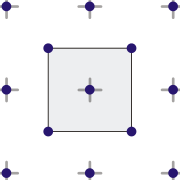
\includegraphics[width=\textwidth]{Plantilla-TFG-master/img/aa5.png}
        \caption{HRAA}
    \end{subfigure}
    \hfill
    \begin{subfigure}[b]{0.25\textwidth}
        \centering
        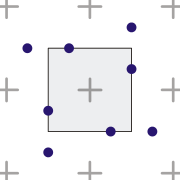
\includegraphics[width=\textwidth]{Plantilla-TFG-master/img/aa6.png}
        \caption{\textit{Flipquad}}
    \end{subfigure}
    \caption{Patrones de supermuestreo \cite{supersamp}}
    \label{fig:patrones}
\end{figure}

Modificar por dónde pasan los rayos dentro de cada píxel equivale a cambiar cómo calculamos los \texttt{uv}. Llamaremos a partir de ahora $AA$ al factor de escalado de la imagen, de forma que por cada píxel haremos pasar $4^{AA}$ rayos. Para hallar los nuevos puntos de muestra bastará con subdividir el píxel en $AA^2$ cuadrantes y quedarnos con el centro de cada uno. Si recordamos que \texttt{gl\_FragCoord} devuelve las coordenadas del centro del píxel, que el ancho y alto del píxel es una unidad, y que tenemos que hacer $AA$ subdivisiones en cada eje, es evidente que podemos obtener los nuevos puntos de muestra desplazando el origen usual del píxel la cantidad
\begin{equation*}
    offset_{m,n} = (m+\nicefrac{1}{2},n+\nicefrac{1}{2}))\cdot subdivision - \left( \frac{lado}{2}, \frac{lado}{2}\right) = \frac{ (m+\nicefrac{1}{2},n+\nicefrac{1}{2}))}{AA} - \left( \frac{1}{2}, \frac{1}{2}\right),
\end{equation*}
donde $m,n\in \{0,\dots, AA-1\}$.\newline
\begin{figure}[!h]
    \centering
    \begin{subfigure}[b]{0.4\textwidth}
        \centering
        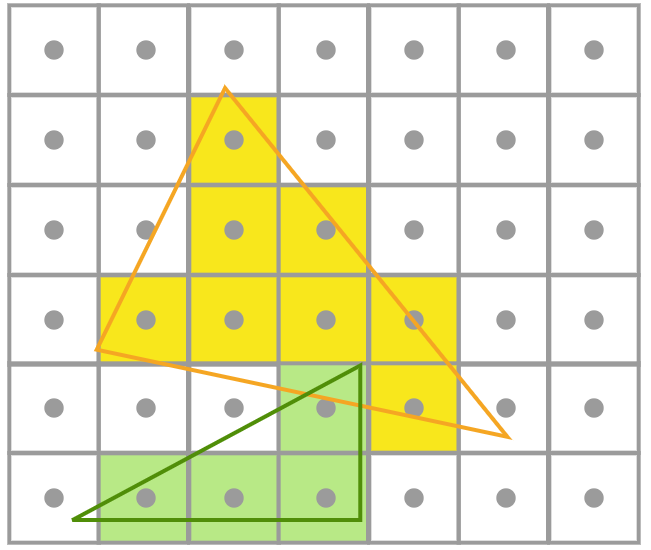
\includegraphics[width=\textwidth]{Plantilla-TFG-master/img/grid1.png}
        \caption{$AA = 1$}
    \end{subfigure}
    \hspace{15pt}
    \begin{subfigure}[b]{0.4\textwidth}
        \centering
        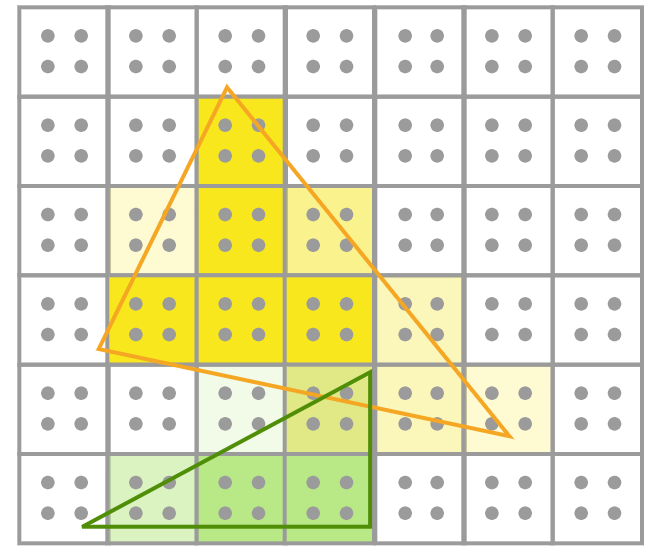
\includegraphics[width=\textwidth]{Plantilla-TFG-master/img/grid2.png}
        \caption{$AA = 2$}
    \end{subfigure}
    \hfill
     \caption{\textit{Antialiasing} para diferentes valores de $AA$}
\end{figure}

Para trasladar esto a nuestro \textit{fragment shader} tan solo habrá que realizar un doble bucle e ir sumando el color obtenido por \textit{spheretracing} en una variable que luego ponderaremos por el número total de muestras, $AA^2$. La nueva versión del \textit{fragment shader} se describe en la \autoref{fig:divPixel}.

\begin{figure}[ht!]
    \centering
    \begin{minipage}{0.69\textwidth}
      \begin{algorithm}[H]
            \caption{Fragment Shader}
            \KwData{posición del observador $c_0$, punto de atención $l$}
            \KwResult{Terna RGBA con el color asignado al píxel actual}
            $color\gets (0,0,0)$
            
            \For{$m \in \{0,\dots, AA-1\}$}{
            \For{$n \in \{0,\dots, AA-1\}$}{
                $offset \gets \frac{(m,n)}{AA} - (0.25, 0.25)$\\[8pt]
                
                $uv \gets 2\cdot \frac{(gl\_FragCoord.xy+offset)- 0.5\cdot u\_resolution.xy}{u\_resolution.y}$\\[8pt]

                $r_d \gets (f_1\ \vert \ f_2\ \vert \ f_3)\cdot normalizar((uv.xy,-1))$\\[5pt]

                $color \gets color + spheretracing(c_0, r_d)$
                }
            }

            $color \gets color / AA^2$
            
            $gl\_FragColor \gets (color, 1)$
        \end{algorithm}
    \end{minipage}%
    \hfill
    \begin{minipage}{0.31\textwidth}
        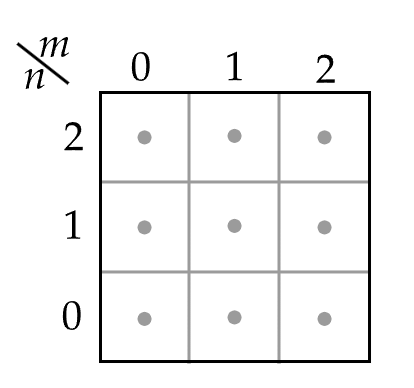
\includegraphics[width=\textwidth]{buclePixels.png}
    \end{minipage}
    \caption{Cuerpo del método \texttt{main} del \textit{fragment shader}}
    \label{fig:divPixel}
\end{figure}

Es evidente que $AA=1$ equivale a no aplicar \textit{antialiasing}, pero tendrá el efecto de desplazar la imagen medio píxel hacia abajo y a la izquierda, pues el único de cada píxel pasará por su esquina inferior. Por tanto, aunque no sea totalmente necesario, se puede añadir una comprobación para calcular los $uv$ como hacíamos originalmente en este caso. En la \autoref{fig:resAA} podemos ver que la pérdida de rendimiento no es en vano y obtenemos una imagen mucho más suave que la original. Sin embargo, no conviene tomar un valor de $AA$ mayor que $3$, pues generará mucha sobrecarga y la mejora no es muy apreciable. Finalmente y para concluir la sección, en el \autoref{ap:comparacionEscenas} podemos ver la construcción que hemos hecho de la escena paso a paso, viendo el efecto que ha tenido en el aspecto final cada técnica que hemos ido añadiendo.

\begin{figure}[htbp]
    \centering
    \begin{subfigure}[b]{0.3\textwidth}
        \centering
        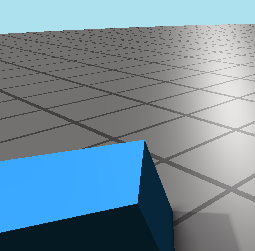
\includegraphics[width=\textwidth]{Plantilla-TFG-master/img/aa1_zoom.png}
        \caption{Detalle con $AA = 1$}
        \label{subfig:noAA}
    \end{subfigure}
    \hfill
    \begin{subfigure}[b]{0.3\textwidth}
        \centering
        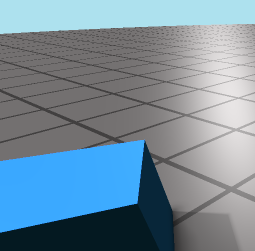
\includegraphics[width=\textwidth]{Plantilla-TFG-master/img/aa2_zoom.png}
        \caption{Detalle con $AA = 2$}
    \end{subfigure}
    \hfill
    \begin{subfigure}[b]{0.3\textwidth}
        \centering
        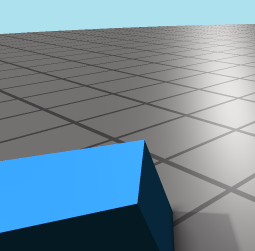
\includegraphics[width=\textwidth]{Plantilla-TFG-master/img/aa3_zoom.png}
        \caption{Detalle con $AA = 3$}
    \end{subfigure}

    \medskip
    
    \begin{subfigure}[b]{\textwidth}
        \centering
        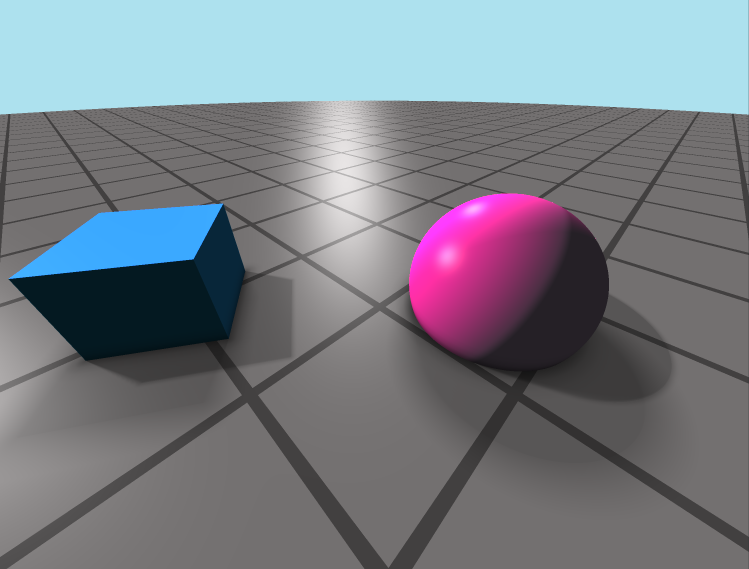
\includegraphics[width=\textwidth]{Plantilla-TFG-master/img/escena9_AA3.png}
        \caption{Escena completa con $AA=3$}
    \end{subfigure}
    
    \caption{Resultados de añadir \textit{antialiasing}}
    \label{fig:resAA}
\end{figure}





